\documentclass{article}
\usepackage[utf8]{inputenc}

\title{Mensa HiQ: De oorsprong van alles.}
\author{Josko de Boer (NL7725)}
\date{December 2016}
\usepackage[square,numbers]{natbib}
\bibliographystyle{abbrvnat}
\usepackage{fourier}
\usepackage{multicol}
\usepackage{fullpage}
\usepackage[dutch]{babel} 
\usepackage[square,numbers]{natbib}
\bibliographystyle{abbrvnat} 
\usepackage{mathrsfs}
\usepackage{amsthm,amsmath,amssymb,amsfonts}  
\usepackage{braket} 
\usepackage{subcaption}
\usepackage{xcolor}
\usepackage{wrapfig}
\usepackage{graphicx}
\renewcommand{\thefootnote}{\Roman{footnote}}
\newcommand{\red}[1]{ {\color{red} #1}}
\date{February 2017} 
\begin{document}
\maketitle
\begin{abstract} 
Een korte introductie in de wetenschappelijke theorie\"en omtrent de oorsprong van alles. Ik ben zelf opgeleid als theoretisch kwantum physicus. Momenteel ben ik een niet-onderzoeker in het lab van Nynke Dekker, waar ik me bemoei met de data analyse van alle onderzoekers.
\end{abstract} 
    \section{Introductie}
     
        \begin{wrapfigure}{r}{.3\textwidth}
            \begin{center}
                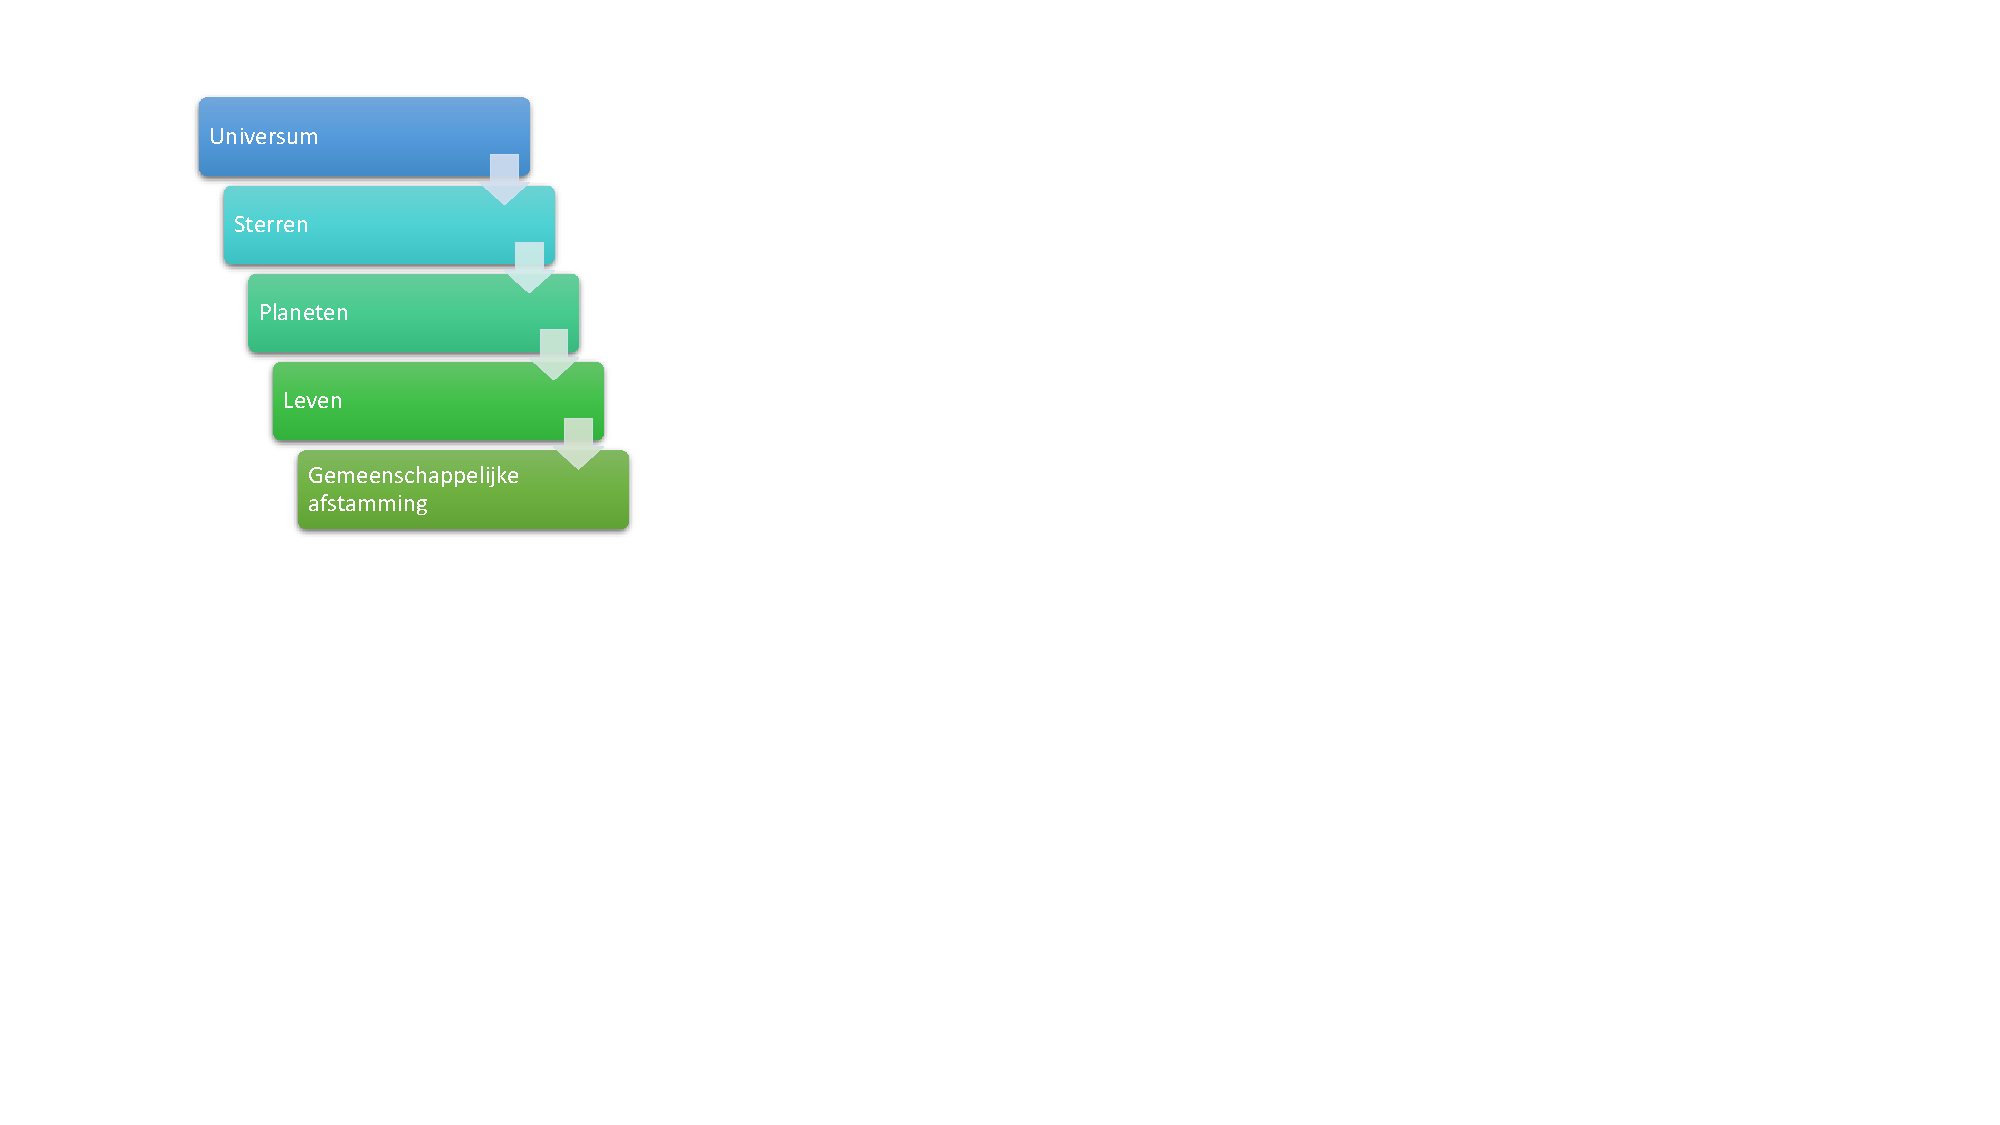
\includegraphics[width=0.29\textwidth, clip, trim=3cm 10cm 23cm 1.5cm]{flowchart}
            \end{center}
            \caption{De onderwerpen die aan bod komen in dit artikel.}
        \end{wrapfigure}
        Op het internet hoor ik vaak kreten zoals 'het is maar een theorie' en 'de wetenschap maakt ook aannames'. Zelden wordt daar nagedacht over wat een wetenschappelijke theorie is, of welke aannames gemaakt worden. Door de groep van wetenschappelijke theorie\"en die \emph{de oorsprong van alles} omschrijven uiteen te zetten, hoop ik hierin het goede voorbeeld te geven.
        
        Wel moeten we het nog kort hebben over de wetenschappelijke methode zelf. De wetenschap is een zoektocht naar kennis over hoe de natuur werkt. Het onderscheidt zich van Filosofie door het rigoureuze experiment. Experimenten zijn primair in deze zoektocht. Vaak wordt er gebruik gemaakt van wiskunde, omdat wiskunde als deductief gereedschap ervoor zorgt dat we onze uitleg kunnen omvormen tot een voorspelling om te testen.   
        
        Sir Isaac Newton formuleerde de vier regels van het wetenschappelijk redeneren in zijn \emph{Principia Mathematica}. De vierde luidt dat een bewering welke uit observatie stamt als accuraat moet worden beschouwd totdat het tegendeel geobserveerd is. Een wetenschappelijke theorie is een groep beweringen welke uitleg geeft aan een verschijnsel. Daarnaast zijn de voorspellingen van deze theorie bevestigd in een experiment en zijn deze te onderscheiden van andere theorie\"en.
    \section{De oorsprong van het Universum}
        Een van de meest bekende wetenschappers was Albert Einstein. Een van zijn grote bijdrages is de \emph{Algemene Relativiteitstheorie} (AR), welke zwaartekracht verklaard als de kromming van ruimte-tijd. Het \emph{kosmologisch principe} stelt dat materie gelijk verdeeld is over het universum. Gecombineerd met relativiteitstheorie leidt dit tot de \emph{Friedmann vergelijkingen}, welke drie oplossingen kennen. Het verschil tussen de oplossingen is meetbaar.
        
        Onder de verschuivingswet van Wien kunnen we de golflengte (kleur) waarop het meeste licht wordt uitgezonden door een ster aan de temperatuur relateren. Maar andere metingen van het meten van de temperatuur van een ster waren het hier absoluut niet mee eens. De roodverschuiving welke gevonden is wordt verklaard omdat het universum \emph{uitdijt}, en de snelheid waarmee dit gebeurt heet de Hubbleconstante. Een universum dat uitdijt is een van de eerder genoemde oplossingen. 
        
        Toen wetenschappers terug in de tijd redeneerden kwam het inzicht dat het kleinere volume van het vroege universum zal leiden tot een veel hogere temperatuur. De uitzetting zal in eerste instantie sneller zijn dan later in het proces, zoals een explosie. Hiervan stamt de naam van het model: \emph{De oerknal}. Dit leidt ook tot de predictie van kosmische achtergrond straling. Deze is inmiddels bevestigd. Andere voorbeelden van bewijs voor dit model zijn de ratio 's van helium, deuterium en lithium, de vormen van galactische stelsels, de verdeling van deze en het bestaan van primordiale gaswolken.
        
    \section{De oorsprong van sterren en planeten}
        Primordiale gaswolken bestaat uit waterstof atomen welke elkaar onderling aantrekken (zwaartekracht). De massa botst tegen elkaar aan, waardoor het deze kracht tegengaat (hitte). Voor een primordiale gaswolk is er zoveel materie dat pure hitte het niet gaat redden. Zwaartekracht wint het van de afstoting van de (negatief) geladen buitenkant van atomen. De elektronen breken los en produceren daarbij hitte. Dit leidt tot een gas van geladen atoomkernen en losse elektronen. Maar zelfs dit is niet genoeg, en zwaartekracht zal de geladen atoomkernen samen brengen in een proces van nucleaire fusie. Hierbij komt weer energie vrij, wat een tijd lang de balans zal houden. Maar op den duur is ook dit weer over, voor een deel omdat deze energie ook weglekt als straling. Het beschreven object is namelijk een zon.
        
        Over zo 'n vijf miljard jaar zal onze zon radicaal veranderen. Wanneer de waterstof kern compleet gefuseerd is tot helium, zal de kern geen hitte meer produceren en daardoor krimpen. Hierdoor worden lagen verder naar buiten dichter, en zal hier ook fusie optreden. De hitte die hierbij vrijkomt laat de zon opzwellen tot een Rode Reus, een gigantische rode zon welke waarschijnlijk groot genoeg is dat de aarde opgeslokt wordt.
        
        De levenscyclus van sterren bevat vele fasen waarin zwaartekracht het uiteindelijk wint van de hitte-opwekkende processen. Hierdoor verschijnen vele elementen. Voor een primordiale gaswolk welke draait, en een deel doet dit, zullen zwaardere elementen naar de buitenkant gecentrifugeerd worden. Het geheel ziet eruit als een schijf.   
        
        Deze protoplanetaire schijf bevat de ingredi\"enten voor een sterrenstelsel zoals het onze. De materie daarin trekt nog altijd elkaar aan, en op de betreffende astronomische tijdschaal zal het zich verzamelen. Dit worden uiteindelijk de planeten \cite{Zhu2015}.
    
    \section{De oorsprong van leven}
    
    \section{Gemeenschappelijke afstamming}
    
    \section{Conclusie}
    \bibliography{referenties}  
\end{document}
